%%
%% This is file `main.tex' based on `sample-sigconf.tex' (q.v. for spurce of that,
%%
%% IMPORTANT NOTICE:
%% 
%% For the copyright see the original source file `sample-sigconf.tex'
%% in the `Sample' folder.
%%
%% For distribution of the original source see the terms
%% for copying and modification in the file samples.dtx.
%% 
%% This generated file may be distributed as long as the
%% original source files, as listed above, are part of the
%% same distribution. (The sources need not necessarily be
%% in the same archive or directory.)
%%
%% Commands for TeXCount
%TC:macro \cite [option:text,text]
%TC:macro \citep [option:text,text]
%TC:macro \citet [option:text,text]
%TC:envir table 0 1
%TC:envir table* 0 1
%TC:envir tabular [ignore] word
%TC:envir displaymath 0 word
%TC:envir math 0 word
%TC:envir comment 0 0
%%
%%
%% The first command in your LaTeX source must be the \documentclass command.

%% NOTE that a single column version is required for 
%% submission and peer review. This can be done by changing
%% the \doucmentclass[...]{acmart} in this template to 
%%\documentclass[manuscript,review,anonymous]{acmart}
%% This version is used for drafting and final submission
\documentclass[sigconf]{acmart}

\usepackage{microtype}
\usepackage{tikz}
\usetikzlibrary{positioning,shapes.multipart}

%% 
%% To ensure 100% compatibility, please check the white list of
%% approved LaTeX packages to be used with the Master Article Template at
%% https://www.acm.org/publications/taps/whitelist-of-latex-packages 
%% before creating your document. The white list page provides 
%% information on how to submit additional LaTeX packages for 
%% review and adoption.
%% Fonts used in the template cannot be substituted; margin 
%% adjustments are not allowed.

%%
%% \BibTeX command to typeset BibTeX logo in the docs
\AtBeginDocument{%
  \providecommand\BibTeX{{%
    \normalfont B\kern-0.5em{\scshape i\kern-0.25em b}\kern-0.8em\TeX}}}

%% Rights management information.  This information is sent to you
%% when you complete the rights form.  These commands have SAMPLE
%% values in them; it is your responsibility as an author to replace
%% the commands and values with those provided to you when you
%% complete the rights form.
%\setcopyright{acmlicensed}
\copyrightyear{2025}
\acmYear{2025}
\acmDOI{}
\setcopyright{none}


%% These commands are for a PROCEEDINGS abstract or paper.
\acmConference[CS-E4780]{CS-E4780 Course Project Evaluation Tables}{October 10,
  2025}{Aalto University}
%
%  Uncomment \acmBooktitle if th title of the proceedings is different
%  from ``Proceedings of ...''!
%
%\acmBooktitle{Woodstock '18: ACM Symposium on Neural Gaze Detection,
%  June 03--05, 2018, Woodstock, NY} 
%\acmISBN{978-1-4503-XXXX-X/18/06}


%%
%% Submission ID.
%% Use this when submitting an article to a sponsored event. You'll
%% receive a unique submission ID from the organizers
%% of the event, and this ID should be used as the parameter to this command.
%%\acmSubmissionID{123-A56-BU3}

%%
%% For managing citations, it is recommended to use bibliography
%% files in BibTeX format.
%%
%% You can then either use BibTeX with the ACM-Reference-Format style,
%% or BibLaTeX with the acmnumeric or acmauthoryear sytles, that include
%% support for advanced citation of software artefact from the
%% biblatex-software package, also separately available on CTAN.
%%
%% Look at the sample-*-biblatex.tex files for templates showcasing
%% the biblatex styles.
%%

%%
%% The majority of ACM publications use numbered citations and
%% references.  The command \citestyle{authoryear} switches to the
%% "author year" style.
%%
%% If you are preparing content for an event
%% sponsored by ACM SIGGRAPH, you must use the "author year" style of
%% citations and references.
%% Uncommenting
%% the next command will enable that style.
%%\citestyle{acmauthoryear}

%%
%% end of the preamble, start of the body of the document source.

%% % Location of your graphics files for figures, here a sub-folder to the main project folder
\graphicspath{{./images/}}

\usepackage{listings}
\usepackage{booktabs}


\begin{document}

%%
%% The "title" command has an optional parameter,
%% allowing the author to define a "short title" to be used in page headers.
\title[Project Report]{Project Report: Enhancing LLM Inference with GraphRAG}


%%
%% The "author" command and its associated commands are used to define
%% the authors and their affiliations.
%% Of note is the shared affiliation of the first two authors, and the
%% "authornote" and "authornotemark" commands
%% used to denote shared contribution to the research.

\author{Daniel Granstr{\"o}m}
\affiliation{%
  \institution{Aalto University}
  \city{Espoo}
  \country{Finland}}
\email{daniel.granstrom@aalto.fi}


\author{Joonatan Korpela}
\affiliation{%
  \institution{Aalto University}
  \city{Espoo}
  \country{Finland}
}
\email{joonatan.korpela@aalto.fi}

\author{Mikael Siidorow}
\affiliation{%
  \institution{Aalto University}
  \city{Espoo}
  \country{Finland}
}
\email{mikael.siidorow@aalto.fi}

%%
%% By default, the full list of authors will be used in the page
%% headers. Often, this list is too long, and will overlap
%% other information printed in the page headers. This command allows
%% the author to define a more concise list
%% of authors' names for this purpose.
\renewcommand{\shortauthors}{Granström, Korpela, Siidorow}

% Project 1 feedback:
% Weak points:
% W1. The report lacks a detailed description of memory utilization measurement. The reported size of 41.7M seems to only reflect the Python objects involved. A more comprehensive description of memory usage would strengthen the analysis.
% W2. The report is shorter than 4 pages. It would benefit from more details on the testbed setup, implementation, and throughput measurement and analysis.


% Please see the weak points as opportunities for improvements for the next course project. Thank you. 

%%
%% The abstract is a short summary of the work to be presented in the
%% article.
\begin{abstract}
  We present a GraphRAG system that enhances LLM inference by integrating knowledge graph retrieval with natural language question answering. The system operates on the Nobel Laureates dataset, translating user questions into Cypher queries executed against an embedded Kuzu graph database. We address two core challenges: improving Text2Cypher accuracy through dynamic few-shot exemplar selection, self-refinement with validation feedback, and rule-based post-processing; and optimizing system performance via LRU caching at the schema pruning and query generation stages. Our ablation study across eight enhancement configurations demonstrates that the combination of few-shot selection and post-processing achieves the best accuracy-latency trade-off, with 100\% syntax validity, 90\% semantic correctness, and average latency under 1.5 seconds. LRU caching reduces end-to-end latency from 1.77 seconds to 6.5 milliseconds on cache hits, a 270x improvement. The implementation and evaluation code are available at \url{https://github.com/dcgran/CS-E4780-project}~\cite{CS-E4780-project}.
\end{abstract}

%%
%% The code below is generated by the tool at: http://dl.acm.org/ccs.cfm
%% Please copy and paste the code instead of the example below.
%%

%% \begin{CCSXML}
%%   <ccs2012>
%%   <concept>
%%   <concept_id>00000000.0000000.0000000</concept_id>
%%   <concept_desc>Do Not Use This Code, Generate the Correct Terms for Your Paper</concept_desc>
%%   <concept_significance>500</concept_significance>
%%   </concept>
%%   <concept>
%%   <concept_id>00000000.00000000.00000000</concept_id>
%%   <concept_desc>Do Not Use This Code, Generate the Correct Terms for Your Paper</concept_desc>
%%   <concept_significance>300</concept_significance>
%%   </concept>
%%   <concept>
%%   <concept_id>00000000.00000000.00000000</concept_id>
%%   <concept_desc>Do Not Use This Code, Generate the Correct Terms for Your Paper</concept_desc>
%%   <concept_significance>100</concept_significance>
%%   </concept>
%%   <concept>
%%   <concept_id>00000000.00000000.00000000</concept_id>
%%   <concept_desc>Do Not Use This Code, Generate the Correct Terms for Your Paper</concept_desc>
%%   <concept_significance>100</concept_significance>
%%   </concept>
%%   </ccs2012>
%% \end{CCSXML}

%% \ccsdesc[500]{Do Not Use This Code~Generate the Correct Terms for Your Paper}
%% \ccsdesc[300]{Do Not Use This Code~Generate the Correct Terms for Your Paper}
%% \ccsdesc{Do Not Use This Code~Generate the Correct Terms for Your Paper}
%% \ccsdesc[100]{Do Not Use This Code~Generate the Correct Terms for Your Paper}

%%
%% Keywords. The author(s) should pick words that accurately describe
%% the work being presented. Separate the keywords with commas.
\keywords{Large Language Models, Retrieval-Augmented Generation}

%% The following are not a requirement, delete if not using
%\received{20 February 2024}  %% inital submission date
%\received[revised]{12 March 2024} %% interim new draft
%\received[accepted]{5 June 2024}  %% publication version

%%
%% This command processes the author and affiliation and title
%% information and builds the first part of the formatted document.
\maketitle

\section{Introduction}

Retrieval-Augmented Generation (RAG) systems enhance Large Language Model (LLM) inference by incorporating external knowledge sources to improve factual accuracy and reduce hallucinations. Traditional RAG approaches rely on semantic similarity search over unstructured text chunks, which works well for many tasks but struggles to capture the rich relational structure underlying complex domains such as scientific collaboration networks, enterprise knowledge bases, and multi-hop reasoning problems. GraphRAG addresses this limitation by integrating graph representations of knowledge into the retrieval process~\cite{han2025retrievalaugmentedgenerationgraphsgraphrag}, enabling LLMs to reason over structured relationships and perform multi-hop queries that would be difficult to express through text-based retrieval alone.

This project implements a GraphRAG system using the Nobel Laureates dataset, which contains mentorship relationships spanning from the 16th century to 2021, enriched with biographical data from the official Nobel Prize API. The dataset is stored in Kuzu, a graph database that supports efficient pattern matching through the Cypher query language. The system pipeline consists of four main stages: schema pruning to identify relevant graph structure, Text2Cypher generation to translate natural language questions into Cypher queries, query execution against the graph database, and response generation by the LLM based on retrieved results.

We address two primary objectives in this work. First, we enhance the Text2Cypher component to improve query generation accuracy through dynamic few-shot exemplar selection, self-refinement with validation feedback, and rule-based post-processing. Second, we optimize system performance through LRU caching and conduct comprehensive benchmarking to characterize latency across all pipeline stages.

Our evaluation includes an ablation study examining all meaningful combinations of Text2Cypher enhancements, quantifying the accuracy-latency trade-offs inherent in each approach. We measure both syntax correctness and semantic correctness against a diverse test set, and analyze cache performance under different workload patterns. The results provide practical insights into which optimizations yield the best balance between response quality and system efficiency.

The remainder of this report is organized as follows. Section~\ref{sec:architecture} describes the system architecture and design decisions. Section~\ref{sec:implementation} details the implementation of both tasks, including testbed setup and measurement methodology. Section~\ref{sec:evaluation} presents our experimental evaluation with comprehensive performance analysis. Section~\ref{sec:discussion} discusses key findings and lessons learned, and Section~\ref{sec:conclusion} concludes.


\section{System Architecture}
\label{sec:architecture}

\subsection{GraphRAG Pipeline}
\label{sec:pipeline}

Our GraphRAG system implements a five-stage pipeline that transforms natural language questions into structured graph queries and generates contextually grounded responses. Figure~\ref{fig:pipeline} illustrates the complete workflow.

\begin{figure*}
  \centering
  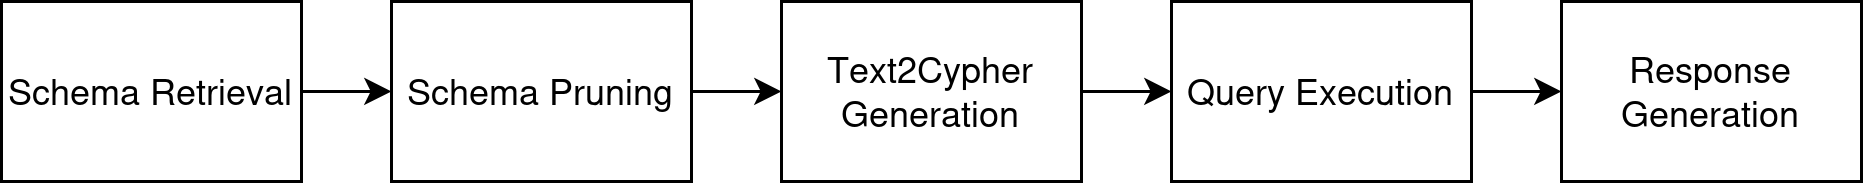
\includegraphics[width=0.6\linewidth]{images/GraphRAG-pipeline.png}
  \caption{Flowchart depicting the complete workflow of the GraphRAG pipeline}
  \Description{A flowchart showing the five stages of the GraphRAG pipeline: Schema Retrieval extracts the graph structure, Schema Pruning filters relevant schema elements, Text2Cypher generates a Cypher query from the user question, Query Execution runs the query against Kuzu, and Response Generation synthesizes the final answer using the LLM.}
  \label{fig:pipeline}
\end{figure*}

\textbf{Stage 1: Schema Retrieval.} The system begins by extracting the complete graph schema from Kuzu, including all node types, relationship types, and their associated properties. This schema provides a comprehensive structural description of the knowledge graph that will be used in subsequent stages.

\textbf{Stage 2: Schema Pruning.} Given a user question, the system uses an LLM to identify which subset of the schema is relevant to answering that question. This pruning step reduces the context size for downstream stages, improving both accuracy and latency.

\textbf{Stage 3: Text2Cypher Generation.} The pruned schema and user question are passed to the Text2Cypher component, which generates a syntactically and semantically valid Cypher query. This stage incorporates three enhancement mechanisms (detailed in Section~\ref{sec:task1}): similarity-based few-shot exemplar selection, self-refinement with validation feedback, and rule-based post-processing.

\textbf{Stage 4: Query Execution.} The generated Cypher query is executed against the Kuzu database. Kuzu's columnar storage and optimized query engine enable efficient pattern matching over the graph structure. The query results are returned as structured data (e.g., lists of nodes, relationships, or aggregated values).

\textbf{Stage 5: Response Generation.} Finally, an LLM synthesizes a natural language response based on the original question, the generated query, and the structured results from the database. This stage translates the retrieved facts into a coherent, human-readable answer that directly addresses the user's information need.

% Placeholder for pipeline diagram
% \begin{figure}[t]
%   \centering
%   \includegraphics[width=\columnwidth]{pipeline.pdf}
%   \caption{GraphRAG pipeline showing the five stages from user question to natural language response. Cache lookup occurs at Stage 3 for previously seen question-schema combinations.}
%   \label{fig:pipeline}
% \end{figure}

\subsection{Knowledge Graph Schema}
\label{sec:schema}

The Nobel Laureates knowledge graph represents prize winners, their institutional affiliations, and geographic metadata. The graph is constructed from the official Nobel Prize API, which provides biographical and institutional data for laureates from 1901 to 2021. Figure~\ref{fig:schema} illustrates the complete schema with all node types and properties.

The schema defines six node types: \textbf{Scholar} (laureate biographical data), \textbf{Prize} (award year, category, motivation, amount), \textbf{Institution} (affiliated organizations), and geographic entities \textbf{City}, \textbf{Country}, and \textbf{Continent}. Seven relationship types connect these entities: \texttt{WON} (Scholar$\rightarrow$Prize), \texttt{BORN\_IN} and \texttt{DIED\_IN} (Scholar$\rightarrow$City), \texttt{AFFILIATED\_WITH} (Scholar$\rightarrow$Institution), \texttt{IS\_LOCATED\_IN} (Institution$\rightarrow$City), and the geographic hierarchy \texttt{IS\_CITY\_IN} (City$\rightarrow$Country) and \texttt{IS\_COUNTRY\_IN} (Country$\rightarrow$Continent).

This structure enables multi-hop queries such as: \textit{``How many Physics laureates were born in European countries?''} or \textit{``Which institutions with Chemistry winners are in the United States?''}

\begin{figure*}[t]
  \centering
  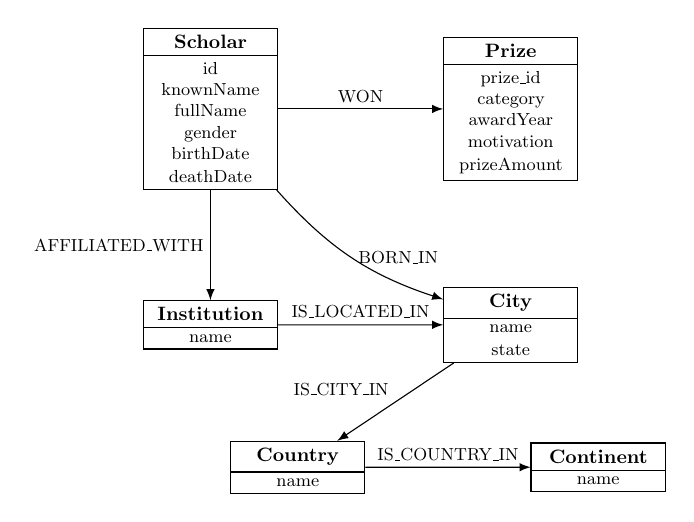
\begin{tikzpicture}[
      scale=0.7,
      every node/.style={transform shape},
      class/.style={rectangle split, rectangle split parts=2, draw, text width=2.2cm, align=center},
      arrow/.style={->,>=latex}
    ]

    % Top row: Scholar and Prize
    \node[class] (scholar) {
      \textbf{Scholar}
      \nodepart{second}
      {\small id\\ knownName\\ fullName\\ gender\\ birthDate\\ deathDate}
    };

    \node[class, right=3cm of scholar] (prize) {
      \textbf{Prize}
      \nodepart{second}
      {\small prize\_id\\ category\\ awardYear\\ motivation\\ prizeAmount}
    };

    % Middle row: Institution and City
    \node[class, below=2cm of scholar] (institution) {
      \textbf{Institution}
      \nodepart{second}
      {\small name}
    };

    \node[class, right=3cm of institution] (city) {
      \textbf{City}
      \nodepart{second}
      {\small name\\ state}
    };

    % Bottom row: Country and Continent
    \node[class, below left=2cm of city] (country) {
      \textbf{Country}
      \nodepart{second}
      {\small name}
    };

    \node[class, right=3cm of country] (continent) {
      \textbf{Continent}
      \nodepart{second}
      {\small name}
    };

    % Relationships
    \draw[arrow] (scholar) -- node[above] {\small WON} (prize);
    \draw[arrow] (scholar) -- node[left] {\small AFFILIATED\_WITH} (institution);
    \draw[arrow] (scholar) to[bend right=15] node[right] {\small BORN\_IN} (city);
    \draw[arrow] (institution) -- node[above] {\small IS\_LOCATED\_IN} (city);
    \draw[arrow] (city) -- node[above left] {\small IS\_CITY\_IN} (country);
    \draw[arrow] (country) -- node[above] {\small IS\_COUNTRY\_IN} (continent);

  \end{tikzpicture}
  \caption{Knowledge graph schema showing node types and relationships in the Nobel Laureates dataset. The schema supports multi-hop queries across prize winners, their institutional affiliations, and hierarchical geographic locations.}
  \Description{A directed graph diagram showing six entity types (Scholar, Prize, Institution, City, Country, Continent) as boxes with their properties listed inside. Arrows connect the entities showing relationships: Scholar connects to Prize via WON, Scholar connects to Institution via AFFILIATED_WITH, Scholar connects to City via BORN_IN, Institution connects to City via IS_LOCATED_IN, City connects to Country via IS_CITY_IN, and Country connects to Continent via IS_COUNTRY_IN.}
  \label{fig:schema}
\end{figure*}

\subsection{Component Interactions}
\label{sec:components}

The system follows a separation of concerns design with three main components: the core GraphRAG pipeline (question-to-answer flow), supporting modules (schema handling, few-shot retrieval, validation, caching), and benchmarking tools (accuracy and latency measurement). The core GraphRAG module orchestrates the pipeline stages, while the database manager handles connections and schema extraction, and DSPy components define structured prompts for pruning, query generation, and answer synthesis. This separation keeps the core logic simple and allows the evaluation scripts to run multiple configurations without modifying the pipeline. Strongly typed schema objects help guide the LLM toward valid outputs.

\section{Implementation}
\label{sec:implementation}

\subsection{Testbed Setup}
\label{sec:testbed}

\textbf{Hardware Environment.} Experiments were conducted on a machine with [TODO: CPU model], [TODO: RAM] GB of memory, running [TODO: OS]. However, hardware specifications have limited impact on end-to-end latency in this system, as the LLM inference---which dominates execution time---is performed remotely via API calls rather than locally.

\textbf{Software Environment.} The system is implemented in Python 3.13 using the following key dependencies:
\begin{itemize}
  \item \textbf{Kuzu} (v0.11.1): Embedded graph database supporting the Cypher query language, used for storing and querying the Nobel Laureates knowledge graph.
  \item \textbf{DSPy} (v3.0.1): Framework for building LLM-powered pipelines with structured prompts, used to orchestrate schema pruning, query generation, and answer synthesis.
  \item \textbf{Sentence Transformers} (v3.0.0): Provides the \texttt{all-MiniLM-L6-v2} embedding model for computing semantic similarity in KNN-based few-shot exemplar selection.
  \item \textbf{cachetools} (v6.1.0): Implements the LRU cache for storing query generation results.
\end{itemize}

\textbf{LLM Configuration.} All LLM inference is performed via the OpenRouter API using the \texttt{google/gemini-2.5-flash} model. This remote inference setup means that observed latencies are influenced by network conditions and API response times, which introduces variability across runs. We mitigate this by averaging results over multiple executions.

\textbf{Test Query Dataset.} We evaluate the system using a benchmark suite of 10 natural language questions designed to cover diverse query patterns:
\begin{itemize}
  \item \textit{Entity lookup}: ``Who won the Nobel Prize in Physics in 2020?''
  \item \textit{Multi-hop with constraints}: ``Which scholars won prizes in Physics and were affiliated with University of Cambridge?''
  \item \textit{Aggregation}: ``How many Nobel Prizes have been awarded in Chemistry?''
  \item \textit{Geographic filtering}: ``List all Nobel Prize winners from Sweden.''
  \item \textit{String matching}: ``Find all scholars whose name contains `Einstein'.''
  \item \textit{Adversarial queries}: Questions designed to stress-test the system, such as ``List Nobel laureates born in Sweden and located in Paris'' (requires correct join semantics) and ``Which laureates winning literature prizes are affiliated with Stanford but not Cambridge?'' (references non-existent prize category).
\end{itemize}
One query is duplicated to measure cache hit behavior. The adversarial queries help identify failure modes in query generation and schema understanding.

\subsection{Task 1: Text2Cypher Enhancement}
\label{sec:task1}

\textbf{Dynamic Few-Shot Exemplar Selection.} We implement dynamic exemplar selection using K-nearest neighbors (KNN) retrieval over a trainset of 15 curated question-query pairs covering diverse query patterns. At inference time, the user's question is embedded using Sentence Transformers (\texttt{all-MiniLM-L6-v2}), and the $k=3$ most similar examples are retrieved and included as few-shot context. This is implemented via DSPy's \texttt{KNNFewShot} optimizer. We also support a static baseline that always selects the first $k$ examples for comparison.

\textbf{Self-Refinement Loop.} We implemented a self-refinement loop that improves the generated Cypher query until it passes a validation check. The validation works by running EXPLAIN <query> on the generated query, and the query is accepted if it does not raise an error. It also ensures that the answer is not a hard-coded string, e.g., RETURN "Cannot answer". The self-refinement loop is run a maximum of 3 times, after which it rejects the query.

\textbf{Rule-Based Post-Processing.} After query generation, we apply regex-based transformations to convert string equality checks into case-insensitive CONTAINS patterns (e.g., \texttt{s.name = 'Einstein'} becomes \texttt{lower(s.name) CONTAINS 'einstein'}). This handles case mismatches and partial string matches on properties like \texttt{name}, \texttt{fullName}, and \texttt{category}.

\subsection{Task 2: Caching and Performance}
\label{sec:task2}

\textbf{LRU Cache Design.} We implement caching at two stages of the pipeline using the \texttt{cachetools.LRUCache} data structure with a maximum capacity of 128 entries each. The first cache stores schema pruning results, avoiding repeated LLM calls when the same question is asked against the same graph schema. The second cache stores generated Cypher queries, eliminating redundant query generation for previously seen question-schema combinations.

Cache keys are computed as a composite of question and schema hashes. Specifically, we compute the MD5 hash of the question text and the MD5 hash of the serialized schema, then concatenate the first 8 hexadecimal characters of each to form a key in the format \texttt{<q\_hash>\_<s\_hash>}. This design ensures that identical questions produce cache hits only when the underlying schema is also unchanged, which is important for correctness when the graph structure evolves. The caches are scoped to each \texttt{GraphRAG} instance rather than shared globally, which prevents warm-cache effects from contaminating benchmark comparisons across different enhancement configurations.

\textbf{Benchmarking Infrastructure.} [TODO: Describe the benchmarking setup, how timing data is collected, and how results are aggregated.]

\textbf{Memory Measurement.} [TODO: Describe memory measurement methodology if applicable.]

\section{Performance Evaluation}
\label{sec:evaluation}

\subsection{Task 1: Text2Cypher Accuracy and Latency}
\label{sec:eval-task1}

Using the benchmark suite described in Section~\ref{sec:testbed}, we evaluate 8 enhancement configurations covering entity lookup, multi-hop reasoning, boolean constraints, and schema disambiguation queries. Table~\ref{tab:ablation} presents the ablation study showing accuracy-latency trade-offs. The Few-shot + Post-processing setting provided the best overall balance, achieving 100\% success and syntax validity, 90\% semantic correctness, and the lowest average latency (~1.43 s). The All refinements configuration performed similarly but at a slightly slower average latency (~1.61 s), which suggests that the additional refinement steps add overhead without improving the quality of the query's semantics.

The baseline configuration was clearly the worst, as it achieved only 80\% across all correctness metrics and was more than three times slower than the best performing configurations. The self refinement only configuration was also inefficient, since while it maintained 100\% success and validity with 90\% semantic correctness, its average latency rose to ~11.32 seconds. This is probably because of it running the expensive query generation multiple times.

All configurations except the baseline were able to produce a semantically correct query for 9 out of the 10 prompts. The only query that proved difficult was "List Nobel laureates born in Sweden and located in Paris." This is because the generated queries either connect Paris to the birth city or use a union instead of an intersection, and they don’t include the expected edge is\_located\_in.

\begin{table*}
  \caption{Ablation Study - Accuracy vs Latency Trade-offs}
  \label{tab:ablation}
  \begin{tabular}{lcccc}
    \toprule
    Configuration                & Syntax Correct (\%) & Semantic Correct (\%) & Avg Latency (ms) & Avg Iterations \\
    \midrule
    Baseline (static few-shot)   & 80                  & 80                    & 4728             & -              \\
    Only Few-shot selection      & 100                 & 90                    & 6494             & -              \\
    Only Self-refinement         & 100                 & 90                    & 11316            & 1.0            \\
    Only Post-processing         & 90                  & 90                    & 1600             & -              \\
    Few-shot + Post-processing   & 100                 & 90                    & 1430             & -              \\
    Few-shot + Refinement        & 100                 & 90                    & 2043             & 0.9            \\
    Refinement + Post-processing & 100                 & 90                    & 2189             & 1.0            \\
    \textbf{All enhancements}    & \textbf{100}        & \textbf{90}           & \textbf{1610}    & \textbf{0.9}   \\
    \bottomrule
  \end{tabular}
\end{table*}

\begin{table*}
  \caption{Pipeline Stage Latency Breakdown With All Refinements (ms)}
  \label{tab:latency}
  \begin{tabular}{lccc}
    \toprule
    Stage               & Without Cache   & With Cache Hit \\
    \midrule
    Schema Pruning      & 1447,3          & 0,0            \\
    Text2Cypher         & 121,7           & 0,1            \\
    Query Execution     & 4,4             & 2,6            \\
    Response Generation & 199,0           & 3,8            \\
    \textbf{Total}      & \textbf{1772,4} & \textbf{6,5}   \\
    \bottomrule
  \end{tabular}
\end{table*}

\subsection{Task 2: Performance and Efficiency}
\label{sec:eval-task2}

Table~\ref{tab:latency} shows the pipeline stage latency breakdown. It was generated using a separate script that aggregates the data from the benchmarking suite. From the table, we can see that there is a significant difference between cold runs and cache hits. Schema pruning, which is normally the slowest step, drops from about 1.45 seconds to essentially zero when cached. Query generation shows a similar pattern, falling from 121.7 ms to 0.1 ms. Response generation also becomes much faster, though not fully eliminated, and query execution sees only a small improvement. Together, these changes reduce end-to-end latency from 1.77 seconds to just 6.5 ms on cache hits.

In cold runs, schema pruning is the clear bottleneck, as it is responsible for more than 80\% of the total latency. Response generation and query synthesis are next, while database execution remains negligible. However, on cache hits, the effect of pruning and query generation on the latency pretty much disappear, and the remaining time comes mostly from lightweight response formatting and a few milliseconds of query execution.

\begin{itemize}
  \item [TODO: Cache hit rate analysis]
  \item [TODO: Performance visualization (flamegraph/bar chart)]
\end{itemize}

\section{Discussion}
\label{sec:discussion}

The key insight from our ablation study is that lightweight techniques---few-shot selection and post-processing---outperform expensive self-refinement while achieving comparable accuracy. Self-refinement's validation loop is most valuable for complex multi-hop queries, but its latency cost (11+ seconds) makes it impractical as a default. Post-processing provides robust case-insensitive matching at negligible cost, which is critical since entity names often differ between user questions and database values.

A consistent challenge was ambiguous geographic queries. The test case ``List Nobel laureates born in Sweden and located in Paris'' failed across configurations because ``located'' could mean birth location, institution location, or residence---highlighting that Text2Cypher accuracy is bounded by question clarity.

For production deployments, we recommend Few-shot + Post-processing with LRU caching. This achieves 90\% semantic accuracy at minimal latency, with cache hits providing 270x speedup for repeated queries.

\section{Conclusion}
\label{sec:conclusion}

We presented a GraphRAG system addressing Text2Cypher accuracy and performance. For Task 1, we implemented KNN-based few-shot selection, EXPLAIN-based self-refinement, and rule-based post-processing. Our ablation study showed that few-shot selection combined with post-processing achieves the best accuracy-latency trade-off. For Task 2, LRU caching at schema pruning and query generation stages reduces latency from 1.77 seconds to 6.5 milliseconds on cache hits. The practical takeaway is that lightweight post-processing can substitute for expensive iterative refinement, and caching is essential for interactive GraphRAG systems.


%%
%% The acknowledgments section is defined using the "acks" environment
%% (and NOT an unnumbered section). This ensures the proper
%% identification of the section in the article metadata, and the
%% consistent spelling of the heading.
%% \begin{acks}
%%   Acknowledgements go here. Delete enclosing begin/end markers if there are no acknowledgements.
%% \end{acks}

%%
%% The next two lines define the bibliography style to be used, and
%% the bibliography file.
\bibliographystyle{ACM-Reference-Format}
\bibliography{references.bib}

%%
\end{document}
\endinput
%%
%% End of file `main.tex'.
